
\section{Centroids and moment of inertia}

\subsection{Centroids}
\begin{knBox}
    {Expression of centroids}
    We use $\bar{x}$ and $\bar{y}$ to denote the \emph{centroid} of a shape. They are the horizontal and vertical distance about a given \textbf{reference axis}.

    The centroid is the \textbf{centre of mass} of the shape. For an axis that the shape is \emph{symmetric about}, the centroid will be \textbf{on the axis}.

    The centroid is also known as the \emph{first moment of area}.
\end{knBox}
\begin{definition}
    {Centroid of composite shapes}
    The centroid of a shape can be found by:
    \[\bar{x}=\frac{\sum (A_i x_i)}{\sum A_i},\quad \bar{y}=\frac{\sum (A_i y_i)}{\sum A_i}\]
    Where $A_i$ is the area of the composition shape, and $x_i, y_i$ are the distances of the composition shape's centroid from the reference axes.
\end{definition}

\label{sec:momentinertia}
\subsection{Moment of inertia}
\begin{knBox}
    {The reference axis for moment of inertia}
    We measure the moment of inertia about a \textbf{reference axis}. This is because at different points, the moment of inertia will be different. (\emph{Unlike the use of reference axes in centroids, where the reference axes is just relative}).

    For finding the moment of inertia at the centroid, we simply set the reference axis at the centroid.
\end{knBox}
\begin{definition}
    {Moment of inertia / Second moment of area}
    The moment of inertia is a measure of an object's resistance to changes in its rotation, about a reference axis. It is given by:
    \[I_x=\int y^2\:dA,\quad I_y=\int x^2\:dA\]
    Where $x$ and $y$ are the distances from the axis. This units are $m^4$.
\end{definition}
\begin{theorem}
    {Moment of inertia for rectangles}
    The moment of inertia for a rectangle is given by:
    \[I_x=\frac{bh^3}{12},\quad I_y=\frac{hb^3}{12}\]
    Where $b$ is the width of the rectangle, and $h$ is the height of the rectangle. This can be derived by the formulas above.

    It is important that the \textbf{direction} where $b$ extends is \textbf{parallel to the reference axis} (so width $\ne$ longest length)
\end{theorem}
\begin{theorem}
    {Moment of inertia for circles}
    The moment of inertia for a circle is given by:
    \[I_x=I_y=\frac{\pi r^4}{4}\]
    Where $r$ is the radius of the circle.
\end{theorem}
\begin{theorem}
    {Parallel axis theorem}
    The moment of inertia about an axis parallel to a reference axis for a shape is given by:
    \[I_{x'}=I_{x}+Ad^2\]
    Where $A$ is the area of the shape, and $d$ is the distance between the \textbf{reference axis} and the \textbf{parallel axis}.
\end{theorem}
\begin{definition}
    {Moment of inertia for composite shapes}
    The moment of inertia for a composite shape is simply the sum of the moments of inertia of the individual shapes \textbf{about the same axis}. This can be expressed as:
    \[I_x=I_{x1\to\bar{y}} + I_{x2\to\bar{y}},\quad I_y=I_{y1\to\bar{x}} + I_{y2\to\bar{x}}\]
    Related: \hyperref[sec:bendingstress]{Bending stress}
\end{definition}

\section{Bending forces and stress}
\subsection{Internal force in beams}
When we consider the internal forces of a beam, we take a \emph{cross section} and consider the forces acting on it. The internal forces are:
\begin{itemize}
    \item \textbf{Shear force} $V$ is the force acting parallel to the cross-section.
    \item \textbf{Bending moment} $M$ is the moment generated by the variation of forces acting perpendicularly to the cross-section.
\end{itemize}

\begin{definition}
    {Sign convention of internal forces}
    $\{+\circlearrowright\}$ The idea is that if the acting force is relatively \textbf{clockwise} to the cross-section $C$, it is \textbf{positive}.
    The following is the signs of internal forces for a \emph{positive} moment:
    \begin{itemize}
        \item \textbf{V:} $\circlearrowright$ (L $\uparrow$ R $\downarrow$)
        \item \textbf{M:} $\curvearrowright\curvearrowleft$ (sagging moment is \emph{positive})
    \end{itemize}
    \tcblower
    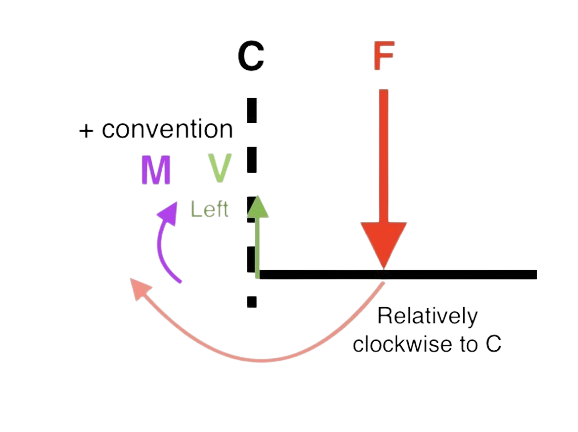
\includegraphics[width=0.33\textwidth]{img/shear2.jpg}
    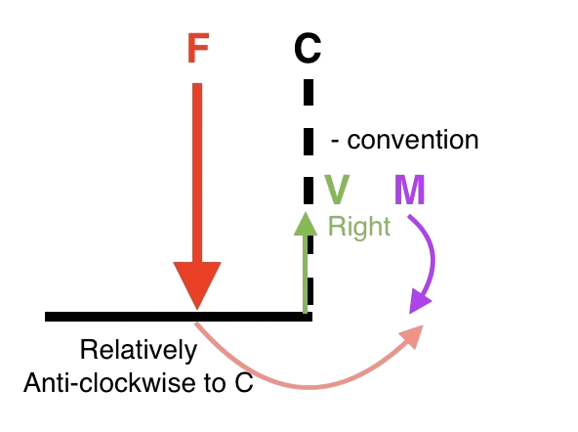
\includegraphics[width=0.33\textwidth]{img/shear1.jpg}

\end{definition}

\begin{knBox}
    {Couple moments}
    When considering couple moments, their effect is \textbf{independent} of the point of application, but they have no effect if they are not in the cut of the beam during analysis. They \textbf{do not exert any force} on the beam, but will affect the reaction forces at supports.
\end{knBox}

\begin{theorem}
    {Finding internal forces by side}
    To find the internal forces at cross-section $C$ \emph{where no loads apply}, we consider the \emph{left} and \emph{right} side of the section:
    \begin{itemize}
        \item \textbf{V:} $\sum F$ on either side
        \item \textbf{M:} $\sum M_C$ on either side about $C$
    \end{itemize}
    Note that the sums are all \textbf{signed by convention}. (e.g. A force $F$ is positive if it points upwards on the left side.)
    
    This also gives us the fact that $\sum F_L =\sum F_R$ and $\sum M_L =\sum M_R$, signed by convention on both sides.
\end{theorem}

\begin{knBox}
    {Finding interal forces on left and right sides}
    To find the interal forces at the left and right cross-section at a point $C$ where loads or moments apply:
    \begin{enumerate}
        \item Left side: $\{\overset{R}{\uparrow}====\overset{V}{\downarrow}\overset{M}{\circlearrowleft}\dots\}$
        \item Right side: $\{\dots\overset{V}{\uparrow}\overset{M}{\circlearrowright}====\overset{R}{\uparrow}\}$
    \end{enumerate}
\end{knBox}

\subsection{Diagramming internal forces}
\begin{definition}
    {Diagramming internal forces}
    The two internal force diagrams are $V(x)-x$ and $M(x)-x$ diagrams. $V(x)$ gives the shear force $V$ at distance $x$ from the \emph{left side} of the beam.
\end{definition}
\begin{theorem}
    {Relation between internal forces}
    The following is the relation between the internal forces:
    \[\frac{dM}{dx}=V\quad \frac{dV}{dx}=-w\]
    Where $w$ is the distributed load acting on the beam.
    \begin{itemize}
        \item This tells us that the slope of the $M(x)$ diagram at an interval is the value of $V$ at that interval.
        \item This tells us that the slope of the $V(x)$ diagram at an interval is the value of $-w$ at that interval.
    \end{itemize}
\end{theorem}

\subsubsection{Steps to follow}
\begin{minipage}{0.6\textwidth}
    \begin{enumerate}
        \item Solve for reaction forces
        \item Draw the FBD of a cut from the leftmost side to a location with distance $x$ from the leftmost force \emph{not analysed}
        \item Analyse the FBD of the cut (solve for $V$ and $M$)
        \item Draw the graphs in the cuts and repeat for all cuts
    \end{enumerate}
\end{minipage}
\hfill
\begin{minipage}{0.35\textwidth}
    \emph{Figurative steps:}
    \begin{enumerate}
        \item $\to R_A, R_B...$
        \item $\{\overset{R}{\uparrow}\ \underbrace{=====}_x\ \overset{V}{\downarrow}\overset{M}{\circlearrowleft}\dots\}$
        \item $\to V, M$
        \item $\to V(x), M(x)$
    \end{enumerate}
\end{minipage}

\vspace{1cm}
To analyse a distributed load $w$, consider the FBD of the whole system on the left, then let $x$ be the distance from the leftmost force \emph{analysed}:

\large
\[\{\underset{\underset{R}{\uparrow}}{=}\underset{2}{==}\overset{\overset{F}{\downarrow}}{=}\underbrace{\overset{\overset{w\cdot x}{\downarrow}}{====}}_x\overset{V}{\downarrow}\overset{M}{\circlearrowleft}\dots\}\]

\subsubsection{Signing conventions}
By convention, we consider the \textbf{positive convention} with respect to the cross-section. That means, if the force is \textbf{clockwise} to the cross-section, it is \textbf{positive}..

\label{sec:bendingstress}
\subsection{Bending stress}
\begin{definition}
    {Pure bending}
    A \textbf{section} of the beam is said to be under \emph{pure bending} if:
    \[V=0,\quad M\text{ constant}\]
\end{definition}
\begin{knBox}
    {Netural axis}
    The neutral axis always \textbf{passes through the centroid} of the beam. It is \emph{netural} as the \textbf{length remains unchanged} for the surface that the axis passes through.

    The distance from the netural axis is denoted $y$ (\textbf{positive downwards}).
\end{knBox}
\begin{knBox}
    {Section modulus}
    The section modulus is given by:
    \[Z=W_z=\frac{I}{y}\]
\end{knBox}
\begin{theorem}
    {Bending stress}
    The bending stress $\sigma$ is given by:
    \[\sigma=\frac{My}{I}\]
    Where $M$ is the bending moment, $y$ is the distance from the \textbf{neutral axis} (centroid), and $I$ is the \textbf{moment of inertia} of the section.

    The formula also tells us that the bending stress is \emph{proportional} to the distance from the neutral axis, and the neutral axis experiences \emph{no stress}.

    Related: \hyperref[sec:momentinertia]{Moment of inertia}
\end{theorem}
\begin{theorem}
    {Maximum tensile and compressive stress}
    \[\sigma^\updownarrow_{max}=\frac{My_\updownarrow}{I}\]
    The maximum tensile and compressive stress $\sigma_{max}$ at a cross section is located at the top $\sigma^\uparrow$  and bottom edge $\sigma^\downarrow$. Note that \textbf{tensile stress is positive} (unlike tension which is negative).
\end{theorem}
